\begin{figure}[!htbp]
\centering
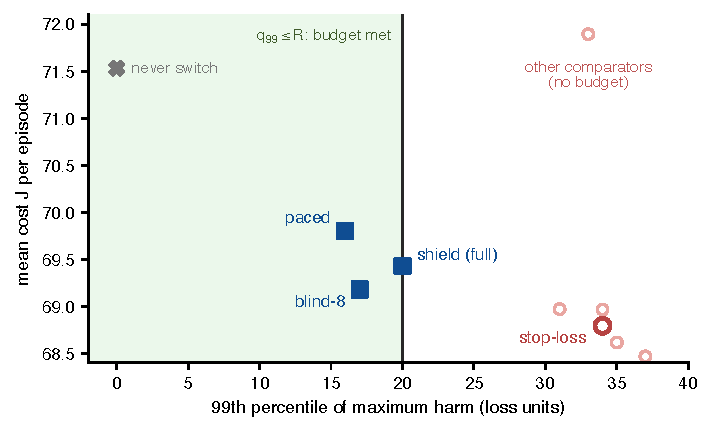
\includegraphics[width=\linewidth]{figures/fig_cost_tail.pdf}
\caption{Tail-risk diagnostic for the registered run (\NRegimes{} regimes, \NSeedsPerRegime{} seeds each): mean cost $J$ against the 99th percentile $q_{99}$ of maximum harm. Panels group arms by budget $R=12,20,30$; the vertical line is $R$ and the shaded region is $q_{99}\le R$. Filled markers satisfy this quantile check; open markers do not, including the stop-loss and the three reserve/width ablations. This 99th-percentile diagnostic does not replace the time-uniform violation guarantee. Never switching has zero harm but pooled $J=\JNever$, about 3 above tuned Wald with cutoff ($J=\JWald$); the budget-free comparators (faint circles: Wald with cutoff, CUSUM, CUSUM rollback, e-process gate) have $q_{99}$ between 31 and 37.}
\label{fig:cost_tail}
\end{figure}
